\documentclass{beamer}
\usepackage{pgfpages}
%\setbeameroption{show notes on second screen=left} %enable for notes
\usepackage{graphicx}
\usepackage{xcolor}
\usepackage{listings}
%\usepackage{transparent}
\usepackage{hyperref}
\lstset{language=python,frame=single}
\usepackage{verbatim}
%\usepackage{apacite}
\usepackage[longnamesfirst]{natbib}
\usepackage{subcaption}
\usepackage{amsmath}
\usepackage{relsize}
\usepackage{appendixnumberbeamer}
\usepackage{xparse}
\usepackage{multimedia}
\usepackage{xcolor}
\usepackage[normalem]{ulem}
\usepackage{tikz}
\usetikzlibrary{matrix,backgrounds}
\usetikzlibrary{positioning}
\usetikzlibrary{shapes,arrows}
\usetikzlibrary{positioning}

\tikzstyle{block} = [rectangle, draw, fill=red!20!blue!10, 
    text width=5em, text centered, rounded corners, minimum height=4em]
\tikzstyle{line} = [draw, line width=1.5pt, -latex']

\pgfdeclarelayer{myback}
\pgfsetlayers{myback,background,main}

\usetheme[numbering=fraction]{metropolis}
%%\AtBeginSection[]
%%{
%%  \begin{frame}
%%    \frametitle{Table of Contents}
%%    \tableofcontents[currentsection]
%%  \end{frame}
%%}

\begin{document}

\title{Toward a theory of transfer}
\author{Andrew Lampinen}
\date{Lightning Talk, Oct. 4th 2017}
\frame{\titlepage}

\begin{frame}{Transfer}
\begin{figure}
\centering
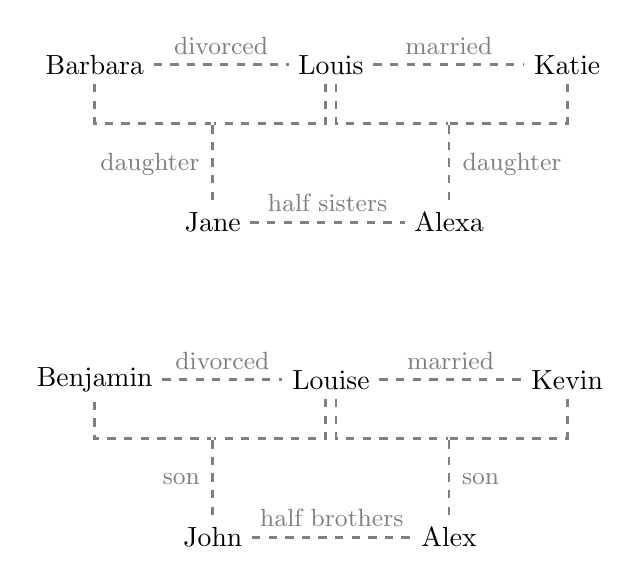
\begin{tikzpicture}[auto]
\node at (0, 0) (Louis) {Louis};  
\node at (-3, 0) (p11) {Barbara};
\path [draw, dashed, opacity=0.5, line width=1.0pt] (p11) -- node {\small divorced} (Louis);

\node at (-1.5, -0.75) [inner sep=0, outer sep=0] (m11) {};
\node at (-1.5, -2) (Jane) {Jane};
\path [draw, dashed, opacity=0.5, line width=1.0pt] (p11) |- (m11);
\path [draw, dashed, opacity=0.5, line width=1.0pt] ([xshift=-0.2cm]Louis) |- (m11);
\path [draw, dashed, opacity=0.5, line width=1.0pt] (m11) -- node [anchor=center, xshift=-0.8cm] {\small daughter} (Jane);

\node at (3, 0) (p12) {Katie};
\path [draw, dashed, opacity=0.5, line width=1.0pt] (Louis) -- node {\small married} (p12);

\node at (1.5, -0.75) [inner sep=0, outer sep=0] (m12) {};
\node at (1.5, -2) (Alexa) {Alexa};
\path [draw, dashed, opacity=0.5, line width=1.0pt] (p12) |- (m12);
\path [draw, dashed, opacity=0.5, line width=1.0pt] ([xshift=0.2cm]Louis) |- (m12);
\path [draw, dashed, opacity=0.5, line width=1.0pt] (m12) -- node [anchor=center, xshift=0.8cm] {\small daughter} (Alexa);
\path [draw, dashed, opacity=0.5, line width=1.0pt] (Jane) -- node {\small half sisters} (Alexa);
\begin{scope}[shift={(0, -4)}]
\node at (0, 0) (Louise) {Louise};  
\node at (-3, 0) (p11) {Benjamin};
\path [draw, dashed, opacity=0.5, line width=1.0pt] (p11) -- node {\small divorced} (Louise);

\node at (-1.5, -0.75) [inner sep=0, outer sep=0] (m11) {};
\node at (-1.5, -2) (John) {John};
\path [draw, dashed, opacity=0.5, line width=1.0pt] (p11) |- (m11);
\path [draw, dashed, opacity=0.5, line width=1.0pt] ([xshift=-0.2cm]Louise) |- (m11);
\path [draw, dashed, opacity=0.5, line width=1.0pt] (m11) -- node [anchor=center, xshift=-0.4cm] {\small son} (John);

\node at (3, 0) (p12) {Kevin};
\path [draw, dashed, opacity=0.5, line width=1.0pt] (Louise) -- node {\small married} (p12);

\node at (1.5, -0.75) [inner sep=0, outer sep=0] (m12) {};
\node at (1.5, -2) (Alex) {Alex};
\path [draw, dashed, opacity=0.5, line width=1.0pt] (p12) |- (m12);
\path [draw, dashed, opacity=0.5, line width=1.0pt] ([xshift=0.2cm]Louise) |- (m12);
\path [draw, dashed, opacity=0.5, line width=1.0pt] (m12) -- node [anchor=center, xshift=0.4cm] {\small son} (Alex);:
\path [draw, dashed, opacity=0.5, line width=1.0pt] (John) -- node {\small half brothers} (Alex);
\end{scope}
\end{tikzpicture}
\note{I'm gonna tell you about a family... Louis is divorced from Barbabara but they have a daughter named Jane, and now Louis is married to Katie}
\end{figure}

{\tiny \citep*{Hinton1986}}
\end{frame}

\begin{frame}{The human condition}
\note{We've suggested that task analogies are much broader than this and may help explain why humans are able to learn so fast.}
\begin{figure}
\centering
\uncover<2->{%
\begin{subfigure}{0.5\textwidth}
\includegraphics[width=\textwidth]{figures/chess_cropped.jpg}
\end{subfigure}}%
\uncover<3->{%
\begin{subfigure}{0.5\textwidth}
\includegraphics[width=\textwidth]{figures/go.jpg}
\end{subfigure}}\\%
\uncover<4->{%
\begin{subfigure}{0.5\textwidth}
\includegraphics[width=\textwidth]{figures/math.jpg}
\end{subfigure}}%
\uncover<5->{%
\begin{subfigure}{0.5\textwidth}
\includegraphics[width=\textwidth]{figures/piano.jpg}
\end{subfigure}}%
\end{figure}
{\tiny \citep*{Hansen2017}}
\end{frame}

\begin{frame}{Neural nets transfer too!}
\begin{figure}
\centering
\begin{tikzpicture}
\node (brain) {\includegraphics[width=0.25\textwidth]{figures/google_brain.jpg}}; 
\node [below = 1cm of brain] (input) {%
\only<2-3>{Ceci n'est pas une pipe.}
\only<5-6>{\includegraphics[width=0.25\textwidth]{figures/un_pipe.jpg}}
};
\node [above = 1cm of brain] (output) {%
\only<3>{This is not a pipe.}
\only<6>{This is a pipe.}
};

\only<2-3,5-6>{
\path [line] (input) -- (brain); 
}
\only<3,6>{
\path [line] (brain) -- (output); 
}
\end{tikzpicture}
\end{figure}
{\tiny \citep*{Luong2016}}
\end{frame}

\begin{frame}[standout]
We suggest these are similar processes.
\end{frame}


\section{Can we make a theory?}

\begin{frame}{Isomorphic tasks for neural networks}

\note{Described tasks that share structure but are not identical, but to make our analysis simpler we are beginning with networks learning two tasks that are truly identical.}
\end{frame}

\begin{frame}<1-5>{Under what conditions?}
\begin{figure}
\centering
\begin{tikzpicture}[auto]
\node [anchor=center, inner sep=0] at (0,0) {\includegraphics[width=\textwidth]{figures/depth_ndom_comp.png}};
\fill<1> [white] (-4.53, 3.18) rectangle (-1.2, 0.2);
\fill<-2> [white] (2.2, 3.18) rectangle (-1.2, 0.2);
\fill<-3> [white] (-4.53, -2.9) rectangle (-1.2, 0.2);
\fill<-4> [white] (2.2, -2.9) rectangle (-1.2, 0.2);
\end{tikzpicture}
\end{figure}

\end{frame}



\section{Wrapping up}

\begin{frame}{Conclusions \& future directions}

\end{frame}

%%\begin{frame}{Acknowledgements}
%%Thanks to:
%%\begin{itemize}
%%    \item Jay McClelland.
%%    \item The rest of the lab.
%%    \item The NSF, for funding.
%%    \item You, for listening. 
%%\end{itemize}
%%\end{frame}

\begin{frame}[standout]
Questions?
\end{frame}

\begin{frame}[allowframebreaks]
\bibliographystyle{plainnat}
{\small \bibliography{shared_reps}}
\end{frame}

\end{document}
